% First we need to tell LaTeX what type of document we'll be writing
\documentclass{article} %lots of other options here, like amsart, among others

% Preamble:

%Here's where packages go. 
\usepackage{amsmath} %includes lots of mathematical symbols and content
\usepackage{lipsum} % For blind text
%\usepackage{fullpage}
%\usepackage[margin=1in]{geometry}
%\usepackage{geometry}
%\geometry{
%  top=1in,
%  inner=1in,
%  outer=1in,
%  bottom=1in,
%}
\usepackage{enumerate}
% incredible building block for diagrams
\usepackage{tikz}
% insertion of imgages
\usepackage{graphicx} 


\usepackage{esint} % Provides \oiint

% PSEUDOCODE package
\usepackage{algorithm}
\usepackage{algpseudocode}
\usepackage{float} % lets us force floats to stay put with [H]

% md framed
\usepackage{mdframed}
\usepackage{hyperref}%%Generally hyperref should be the last package loaded. 
% i did not know this needed to be the last package loaded

\hypersetup{
	   colorlinks=true,
	   urlcolor=blue,
	   linkcolor=black
	}
	
\title{Math 3680: Week 4}
\author{Arjan Singh Ellingson}
%\date{August 24th, 2026}
\date{\today}

\begin{document}

\maketitle
%\tableofcontents

\section{Introduction}\label{sec:Intro}
On its own, \LaTeX is great and producing text. But it is through \emph{packages} that a \LaTeX document can really shine, whether it is including colored text, graphics, or source code from your document. We'll need specific packages for certain topics later, but today is an introduction to packages more broadly.

\section{Including Packages}
Packages are activated in the preamble by the general format
\begin{center}
	{\tt \textbackslash usepackage[<options>]\{<package>\}}.
\end{center}
You can also load multiple packages at once using
\begin{center}
	{\tt \textbackslash usepackage[<options>]\{<package1>,<package2>,\dots\}}.
\end{center}
For example, one instance of {\tt \textbackslash usepackage} I pulled from a random document of mine is
\begin{center}
	{\tt \textbackslash usepackage\{graphicx, amsmath, amssymb, enumerate, mathtools\}}
\end{center}

\section{Updating Your Packages}
Depending on how you use \LaTeX, you may need to manually update your packages in your system. Updates to packages come all the time, so you may wish to set a reminder to update these packages at a regular time interval if not using Overleaf.

\subsection{Overleaf}
If you use Overleaf, it should have the most up-to-date versions of packages.

\subsection{Mac} On a Mac, your packages are likely housed in \emph{TeX Live Utility}. Just search for this program, open it, update your package list, and install all updates.

Arjan edit: I had a lot of packages to update, 2030 to be exact.
\subsection{PC} On a PC, your packages are likely housed in a program called \emph{MiKTeX Console}. Just search for this program, open it, update your package list, and install all updates.

\subsection{Linux} If you're running TeX through Linux or on the Command Line/Terminal, then your options are dependent upon how you installed TeX. If you installed \emph{TeX Live} using a Linux package manager (like {\tt apt} on Ubuntu/Debian or {\tt dnf} on Fedora), {\tt tlmgr} is usually disabled.

\section{Examples}
\subsection{{\tt fullpage} Package}
Comment/uncomment the package above to see what happens!

\subsection{{\tt geometry} Package}
Two instances of this package are shown above. One automatically creates 1-inch margins, while the other gives you the option to change the margins on each side.

\subsection{{\tt enumerate} Package }
This allows you more control over the numbering in lists.
\begin{enumerate}[I) ]
	\item First item
	\item Second item
	      \begin{enumerate}[i)]
		      \item first subitem
	      \end{enumerate}
\end{enumerate}

\subsection{{\tt hyperref} Package}
This package makes your PDF include clickable links. This could be via URLs:
\begin{itemize}
	\item \url{https://www.calpoly.edu} % Clickable and formatted!
	\item \href{https://www.calpoly.edu}{Your favorite university} % Clickable text!
\end{itemize}
Or it could be used to navigate through your document. For example, click \ref{sec:Intro} to return to the first section (see where the {\tt \textbackslash label} command is used??).

% ------- MY ADDITIONS ---------------
\section{MY ADDITIONS!!}
Here is what I am going play with some packages I have had a bit of former experience with. Float package was also used to pin large environments to the source line order.
\subsection{TikZ Package}
I have had lots of experience with the TikZ package, which allows individuals to make fun shapes and graphs in \LaTeX. To make a drawing, encloses \texttt{tikzpicture} environment in \texttt{\textbackslash begin\{tikzpicture\}} and \texttt{\textbackslash end\{tikzpicture\}}.

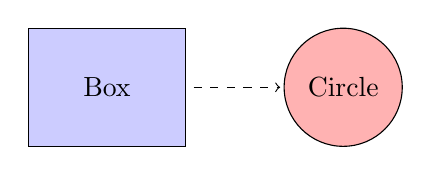
\begin{tikzpicture}
	% Draw a rectangle
	\draw[fill=blue!20] (0,0) rectangle (2,1.5);

	% Draw a circle
	\draw[fill=red!30] (4,0.75) circle (0.75);

	% Arrow
	\draw[->, dashed] (2.1,0.75) -- (3.2,0.75);

	% Add labels
	\node at (1,0.75) {Box};
	\node at (4,0.75) {Circle};

\end{tikzpicture}
I have some code from my notes from a previous class that I will include here.\\
This is the same library just a different subset of code. Here is a graph with four nodes.\\

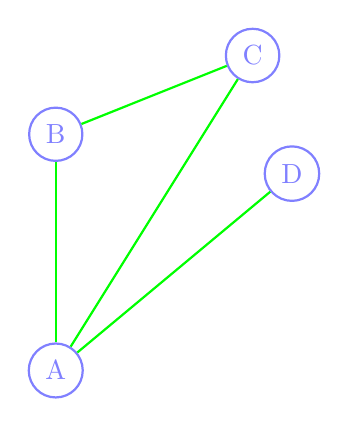
\begin{tikzpicture}[
		every node/.style={circle, draw=blue!50, text=blue!50},
		every path/.style={draw=green, thick}
	]
	\node (A) at (0,0) {A};
	\node (B) at (0,3) {B};
	\node (C) at (2.5,4) {C};
	\node (D) at (3,2.5) {D};
	\draw (D) -- (A);
	\draw (B) -- (A);
	\draw (A) -- (C);
	\draw (C) -- (B);
\end{tikzpicture}

\subsection{Linky Linky}
Here I am just linking a few websites.
\begin{itemize}
	\item \href{https://www.youtube.com/}{Youtube (clicky text)}
	\item \url{https://aselling.us} : This is my website (WIP but fun)
	\item \href{https://aselling-us.github.io/resume/ArjanEllingsonResume.pdf}{LaTeX Resume} This is also my resume, which is formatted in \LaTeX.
\end{itemize}

\subsection{Images!}
Here I now want to include an image. I have an image in the same folder as this file, so they will be inserted here.


\begin{figure}[h]
	\centering
	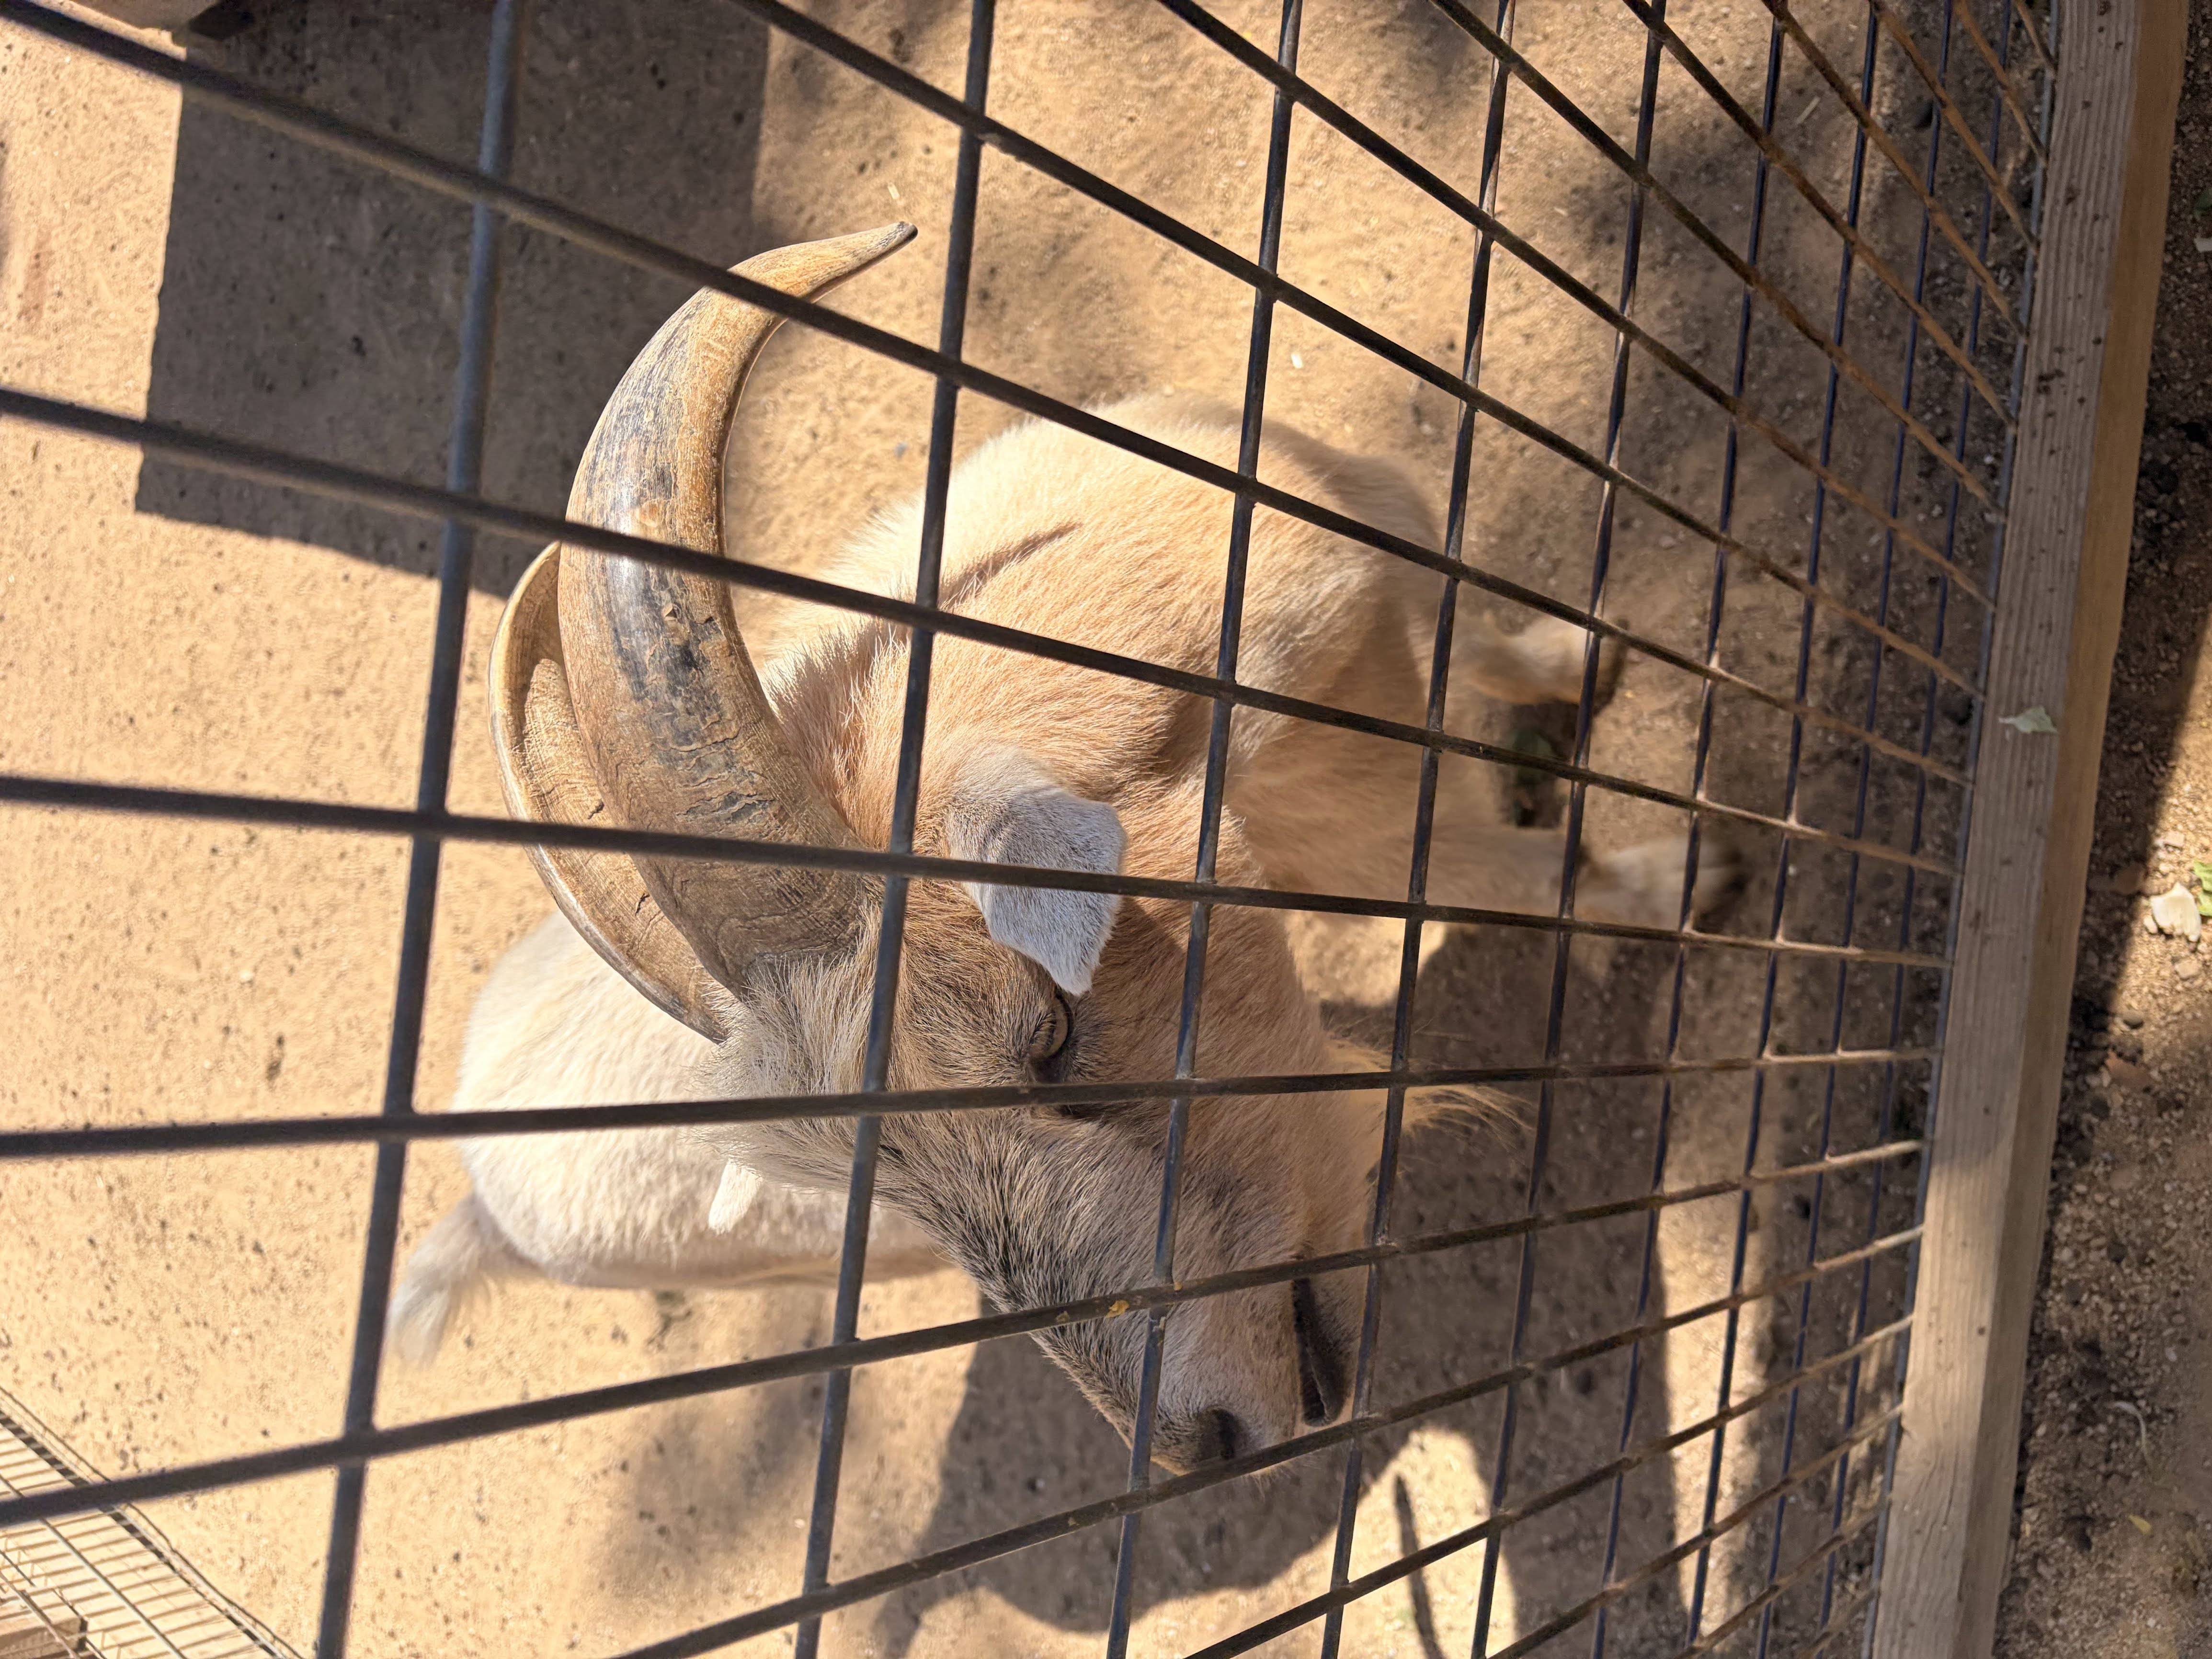
\includegraphics[width=0.8\textwidth, angle=-90]{IMG_0316.jpg}
	\caption{This is a fun photo from this weekend from Avila Farms.}
	\label{fig:img1}
\end{figure}
\subsection{A fun custom integral symbol from esint package}
This package gives access to a few custom integral symbols, including the double integral and triple integral. Here is an example of a closed surface integral symbol:
$$\oiint$$

\subsection{Pseudocode Package}
I have also used the pseudocode package before which allows for nicer formatting of pseudocode. There are two libraries that are used together, the algorithm package and the algpseudocode package. 
This is the pseudocode for the Depth-First Search (DFS) algorithm, which is a graph traversal algorithm.

\begin{algorithm}[H]
\caption{DFS}
\begin{algorithmic}
	\Require A graph $G = (V, E)$.
	\Ensure A labeling of the vertices of $G$ such that every vertex has a "discovered" label set to TRUE. The by product is a \textit{forest} of connect components of $G$.
	\Procedure{DFS}{$G$}
	\For{all $v \in V$}
		\State $discovered(v) = \text{FALSE}$
	\EndFor
	\For{all $v \in V$}
			\If{$discovered(v) = \text{FALSE}$}
				\State \Call{EXPLORE}{$G, v$}
			\EndIf
		\EndFor
	\EndProcedure
	\end{algorithmic}
\end{algorithm}

\subsection{Md-Framed}
This is useful package for theorem and framed environments. Note that it is different than \texttt{amsthm} package.
\begin{mdframed}[frametitle = {Pythagorean Theorem}, style = important]

The Pythagorean Theorem is a method for finding the hypotenuse
\[
a^2 + b^2 = c^2
\]

where $a$ and $b$ are the legs and $c$ is the hypotenuse.

\end{mdframed}
\end{document}












